\documentclass[a4paper,10pt]{article}
\usepackage{graphicx}
\graphicspath{{pics/}}
\begin{document}
\begin{figure}
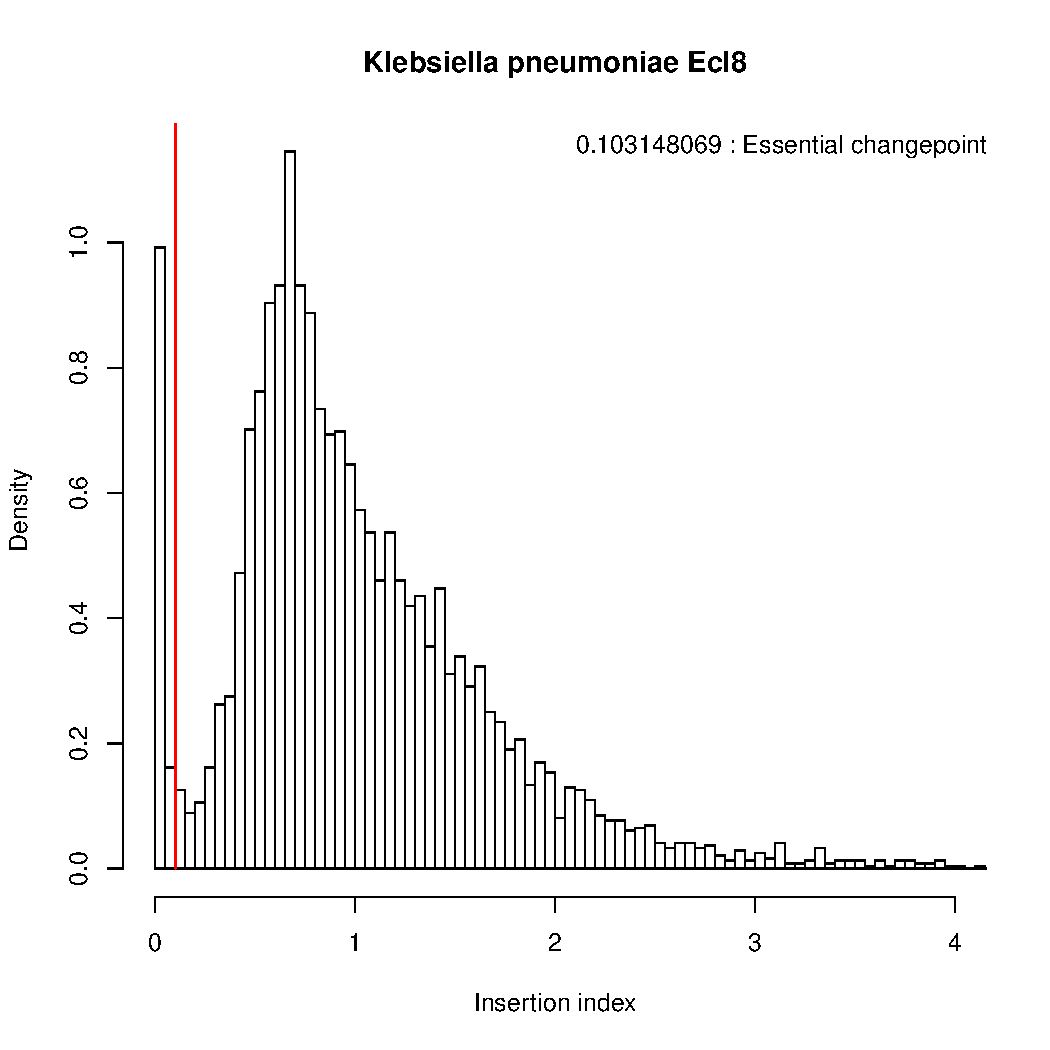
\includegraphics[scale=0.2, page=1]{mixtools-no.pdf}
\includegraphics[scale=0.2, page=2]{mixtools-no.pdf}
\includegraphics[scale=0.2, page=3]{mixtools-no.pdf}\\
\includegraphics[scale=0.2, page=4]{mixtools-no.pdf}
\includegraphics[scale=0.2, page=5]{mixtools-no.pdf}
\includegraphics[scale=0.2, page=6]{mixtools-no.pdf}\\
\includegraphics[scale=0.2, page=7]{mixtools-no.pdf}
\includegraphics[scale=0.2, page=8]{mixtools-no.pdf}
\includegraphics[scale=0.2, page=9]{mixtools-no.pdf}\\
\includegraphics[scale=0.2, page=10]{mixtools-no.pdf}
\includegraphics[scale=0.2, page=11]{mixtools-no.pdf}
\includegraphics[scale=0.2, page=12]{mixtools-no.pdf}
\caption{$ii=\frac{\frac{insertioncites(gene)}{length(gene)}}{\frac{insertioncites(genome)}{length(genome)}}$\newline
\textbf{Method:} gammamixEM \newline
\textbf{trimming:} 5 prime site: 5\%, 3 prime site: 10\%\newline
\textbf{plot manipulations:} Added 0.001 to all numbers \newline
\textbf{Number of essential genes:}\newline
Klebsiella pneumoniae Ecl8: 287\newline
Escherichia coli ETEC CS17: 622\newline
Enterobacter: 344\newline
Klebsiella pneumoniae RH201207: 5579\newline
Escherichia coli ETEC H10407: 460\newline
Escherichia coli UPEC: 365\newline
Citrobacter: 339\newline
Salmonella enteritidis: 380\newline
Salmonella typhimurium SL1344: 428\newline
Salmonella typhimurium D23580: 366\newline
Salmonella typhimurium A130: 413\newline
Salmonella typhi: 568}
\end{figure}

\begin{figure}
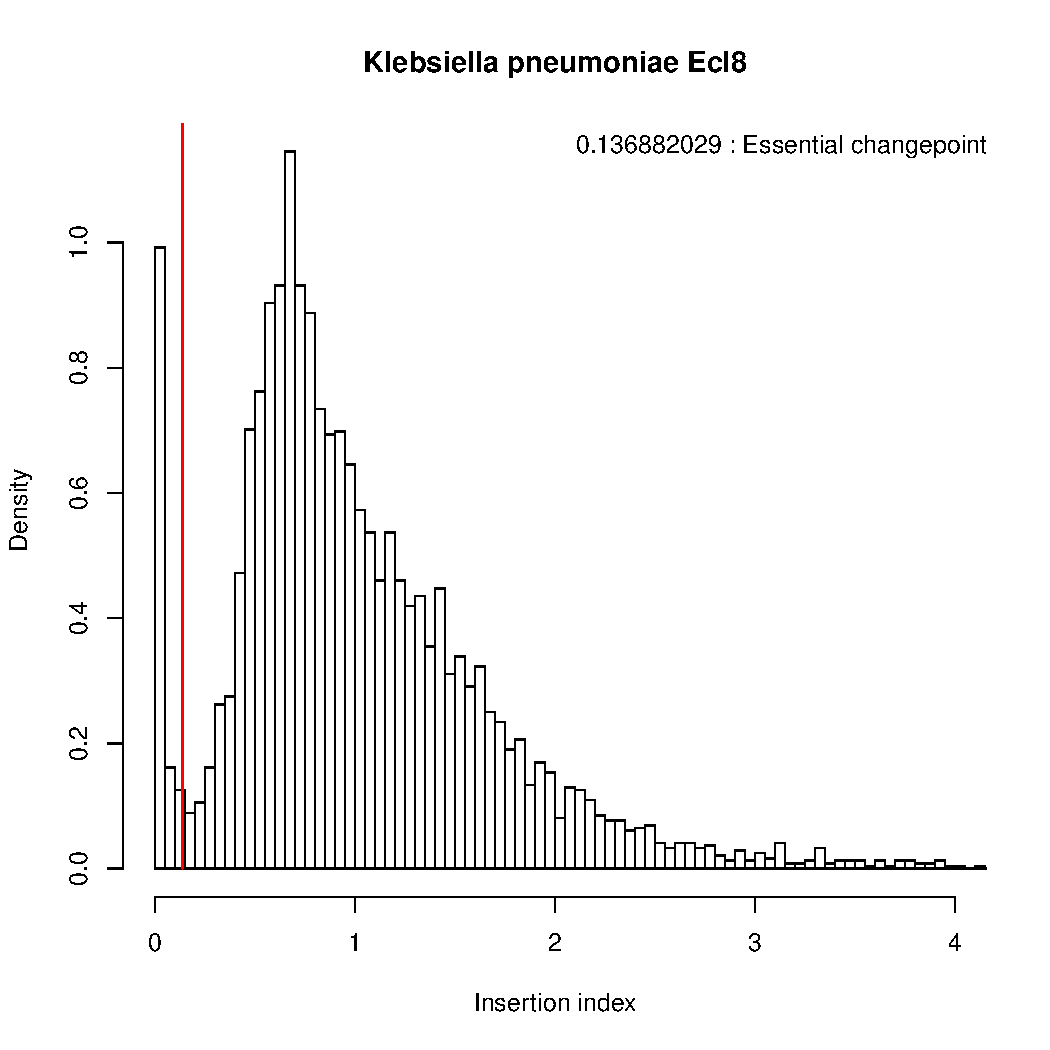
\includegraphics[scale=0.2, page=1]{mixtools-10.pdf}
\includegraphics[scale=0.2, page=2]{mixtools-10.pdf}
\includegraphics[scale=0.2, page=3]{mixtools-10.pdf}\\
\includegraphics[scale=0.2, page=4]{mixtools-10.pdf}
\includegraphics[scale=0.2, page=5]{mixtools-10.pdf}
\includegraphics[scale=0.2, page=6]{mixtools-10.pdf}\\
\includegraphics[scale=0.2, page=7]{mixtools-10.pdf}
\includegraphics[scale=0.2, page=8]{mixtools-10.pdf}
\includegraphics[scale=0.2, page=9]{mixtools-10.pdf}\\
\includegraphics[scale=0.2, page=10]{mixtools-10.pdf}
\includegraphics[scale=0.2, page=11]{mixtools-10.pdf}
\includegraphics[scale=0.2, page=12]{mixtools-10.pdf}
\caption{$ii=\frac{\frac{insertioncites(gene)}{length(gene)}}{\frac{insertioncites(genome)}{length(genome)}}$\newline
\textbf{Method:} gammamixEM \newline
\textbf{trimming:} 5 prime site: 5\%, 3 prime site: 10\%\newline
\textbf{plot manipulations:} Removed the tail after visiting the first bin with frequency less than 10, added 0.001 to all numbers \newline
\textbf{Number of essential genes:}\newline
Klebsiella pneumoniae Ecl8: 310 \newline
Escherichia coli ETEC CS17: 569 \newline
Enterobacter: 2961 \newline
Klebsiella pneumoniae RH201207: 350 \newline
Escherichia coli ETEC H10407: 433 \newline
Escherichia coli UPEC: 307 \newline
Citrobacter: 330 \newline
Salmonella enteritidis: 303 \newline
Salmonella typhimurium SL1344: 411 \newline
Salmonella typhimurium D23580: 316 \newline
Salmonella typhimurium A130: 4094 \newline
Salmonella typhi: 3697}
\end{figure}

\begin{figure}
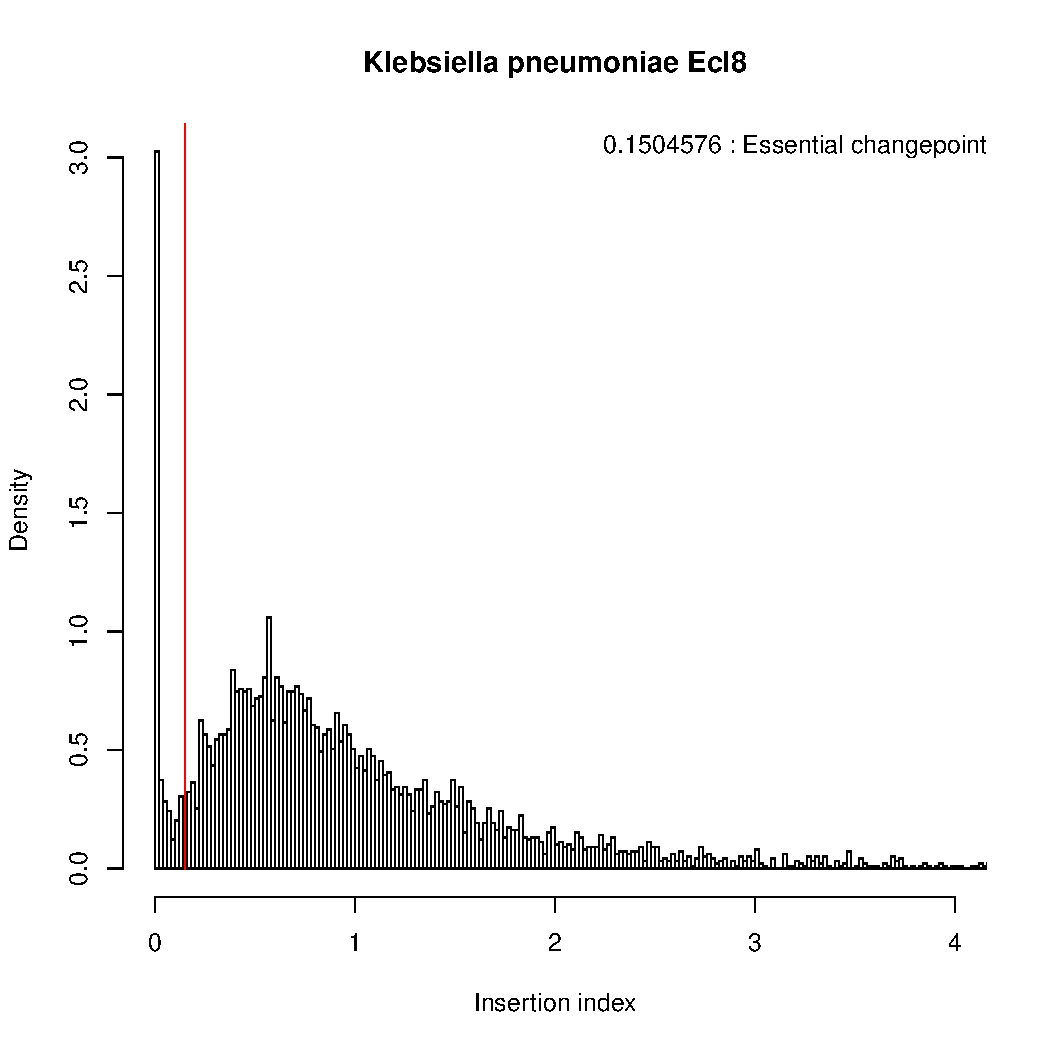
\includegraphics[scale=0.2, page=1]{mixtools-no-reads.pdf}
\includegraphics[scale=0.2, page=2]{mixtools-no-reads.pdf}
\includegraphics[scale=0.2, page=3]{mixtools-no-reads.pdf}\\
\includegraphics[scale=0.2, page=4]{mixtools-no-reads.pdf}
\includegraphics[scale=0.2, page=5]{mixtools-no-reads.pdf}
\includegraphics[scale=0.2, page=6]{mixtools-no-reads.pdf}\\
\includegraphics[scale=0.2, page=7]{mixtools-no-reads.pdf}
\includegraphics[scale=0.2, page=8]{mixtools-no-reads.pdf}
\includegraphics[scale=0.2, page=9]{mixtools-no-reads.pdf}\\
\includegraphics[scale=0.2, page=10]{mixtools-no-reads.pdf}
\includegraphics[scale=0.2, page=11]{mixtools-no-reads.pdf}
\includegraphics[scale=0.2, page=12]{mixtools-no-reads.pdf}
\caption{$ii=\frac{\frac{reads(gene)}{length(gene)}}{\frac{reads(genome)}{length(genome)}}$\newline
\textbf{Method:} gammamixEM \newline
\textbf{trimming:} 5 prime site: 5\%, 3 prime site: 10\%\newline
\textbf{plot manipulations:} Added 0.001 to all numbers \newline
\textbf{Number of essential genes:}\newline
Klebsiella pneumoniae Ecl8: 159 \newline
Escherichia coli ETEC CS17: 87 \newline
Enterobacter: 175 \newline
Klebsiella pneumoniae RH201207: 252 \newline
Escherichia coli ETEC H10407: 569 \newline
Escherichia coli UPEC: 194 \newline
Citrobacter: 145 \newline
Salmonella enteritidis: 1297 \newline
Salmonella typhimurium SL1344: 103 \newline
Salmonella typhimurium D23580: 65 \newline
Salmonella typhimurium A130: 522 \newline
Salmonella typhi: 4321}
\end{figure}

\begin{figure}
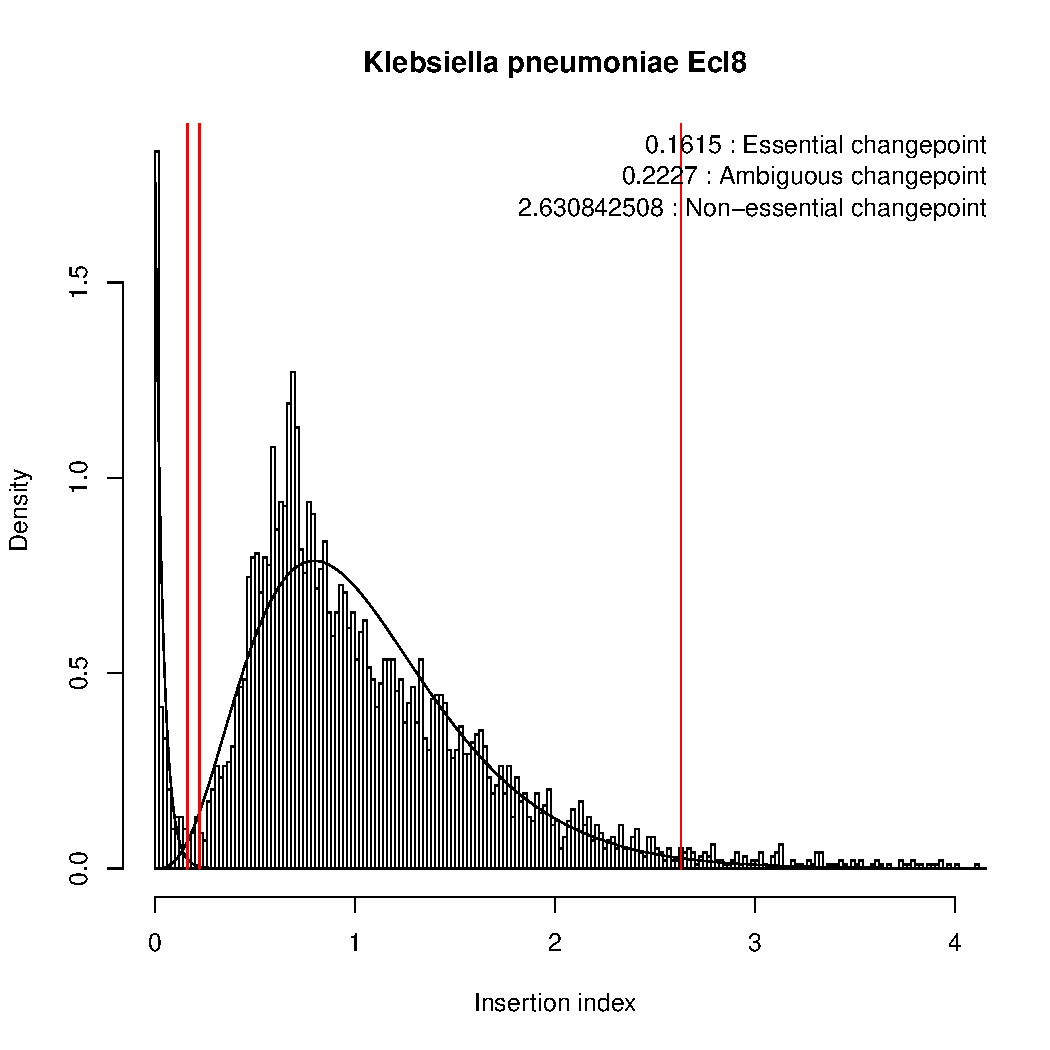
\includegraphics[scale=0.2, page=1]{lars.pdf}
\includegraphics[scale=0.2, page=2]{lars.pdf}
\includegraphics[scale=0.2, page=3]{lars.pdf}\\
\includegraphics[scale=0.2, page=4]{lars.pdf}
\includegraphics[scale=0.2, page=5]{lars.pdf}
\includegraphics[scale=0.2, page=6]{lars.pdf}\\
\includegraphics[scale=0.2, page=7]{lars.pdf}
\includegraphics[scale=0.2, page=8]{lars.pdf}
\includegraphics[scale=0.2, page=9]{lars.pdf}\\
\includegraphics[scale=0.2, page=10]{lars.pdf}
\includegraphics[scale=0.2, page=11]{lars.pdf}
\includegraphics[scale=0.2, page=12]{lars.pdf}
\caption{$ii=\frac{\frac{insertions(gene)}{length(gene)}}{\frac{insertions(genome)}{length(genome)}}$\newline
\textbf{Method:} Lars' method \newline
\textbf{trimming:} 5 prime site: 5\%, 3 prime site: 10\%\newline
\textbf{plot manipulations:} Lars' manipulations
\textbf{Number of essential genes:}\newline
Klebsiella pneumoniae Ecl8: 322 \newline
Escherichia coli ETEC CS17: 528 \newline
Enterobacter: 351 \newline
Klebsiella pneumoniae RH201207: 387 \newline
Escherichia coli ETEC H10407: 429 \newline
Escherichia coli UPEC: 354 \newline
Citrobacter: 330 \newline
Salmonella enteritidis: 285 \newline
Salmonella typhimurium SL1344: 416 \newline
Salmonella typhimurium D23580: 333 \newline
Salmonella typhimurium A130: 357 \newline
Salmonella typhi: 361}
\end{figure}

\begin{figure}
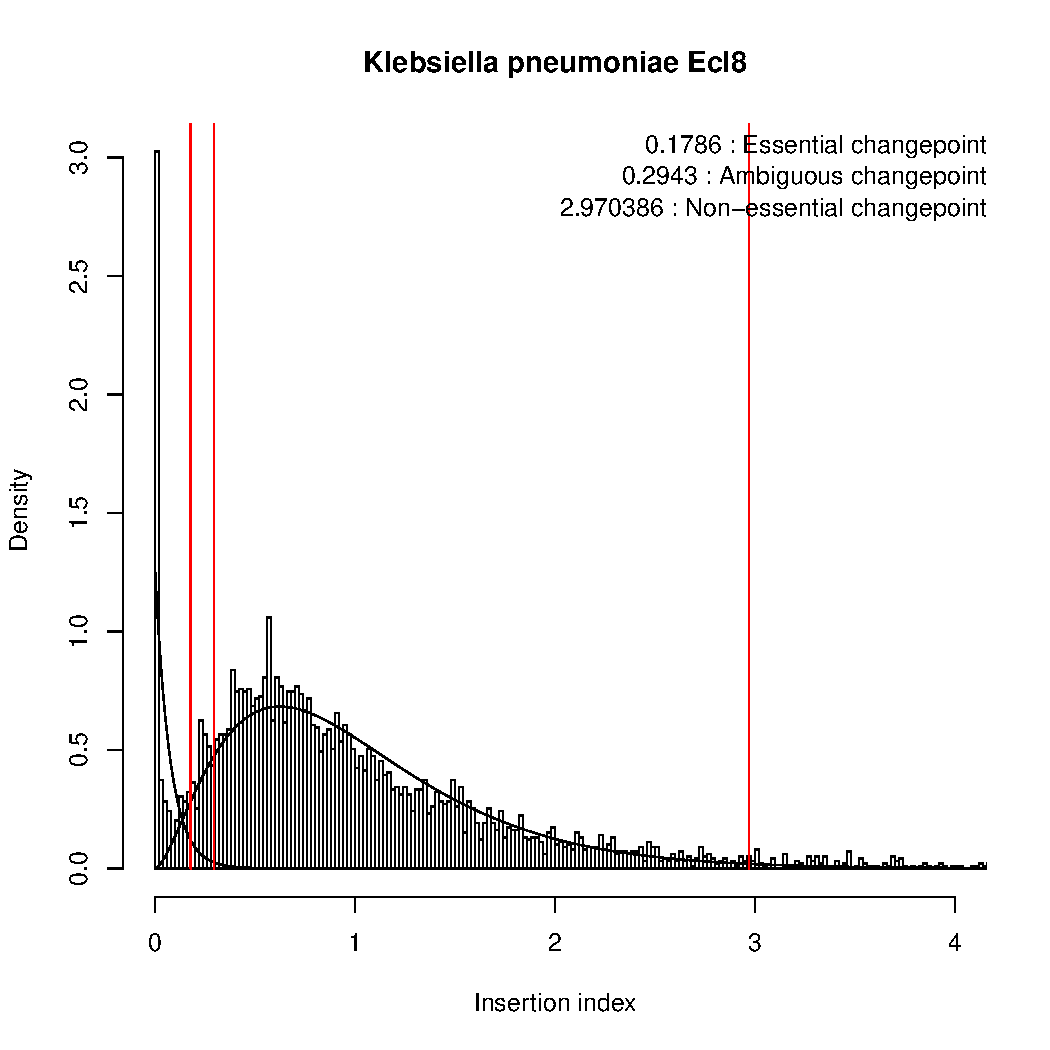
\includegraphics[scale=0.2, page=1]{lars-reads.pdf}
\includegraphics[scale=0.2, page=2]{lars-reads.pdf}
\includegraphics[scale=0.2, page=3]{lars-reads.pdf}\\
\includegraphics[scale=0.2, page=4]{lars-reads.pdf}
\includegraphics[scale=0.2, page=5]{lars-reads.pdf}
\includegraphics[scale=0.2, page=6]{lars-reads.pdf}\\
\includegraphics[scale=0.2, page=7]{lars-reads.pdf}
\includegraphics[scale=0.2, page=8]{lars-reads.pdf}
\includegraphics[scale=0.2, page=9]{lars-reads.pdf}\\
\includegraphics[scale=0.2, page=10]{lars-reads.pdf}
\includegraphics[scale=0.2, page=11]{lars-reads.pdf}
\includegraphics[scale=0.2, page=12]{lars-reads.pdf}
\caption{$ii=\frac{\frac{reads(gene)}{length(gene)}}{\frac{reads(genome)}{length(genome)}}$\newline
\textbf{Method:} Lars' method \newline
\textbf{trimming:} 5 prime site: 5\%, 3 prime site: 10\%\newline
\textbf{plot manipulations:} Lars' manipulations
\textbf{Number of essential genes:}\newline
Klebsiella pneumoniae Ecl8: 322 \newline
Escherichia coli ETEC CS17: 528 \newline
Enterobacter: 351 \newline
Klebsiella pneumoniae RH201207: 387 \newline
Escherichia coli ETEC H10407: 429 \newline
Escherichia coli UPEC: 354 \newline
Citrobacter: 330 \newline
Salmonella enteritidis: 285 \newline
Salmonella typhimurium SL1344: 416 \newline
Salmonella typhimurium D23580: 333 \newline
Salmonella typhimurium A130: 357 \newline
Salmonella typhi: 361}
\end{figure}
\end{document}